\subsection{Question 2(2): Vehicle Reuse and Min--Max Scheduling}\label{sec:q22}

\subsubsection{Model}

Three alerts and six task slots with five vehicles force at least one vehicle to serve
two alerts. A \emph{structure} fixes the discrete decisions: the doubling vehicle
$k$, its ordered alert pair, the partner of the doubled vehicle on its first alert, the
partner on its second alert, and the two vehicles of the remaining alert. Within the
single-doubler family (all five vehicles used, exactly one doubles---Assumption~5) the
count is $5\times3\times2\times4!/2=360$; we declare this family as the search scope and
report optimality evidence relative to it. Each alert must be served by two
\emph{different} vehicles from stations inside its observable region, with the azimuth
guard $\gamma\ge1^\circ$ between the two sightlines.

Given a structure and stations, the event-timeline simulator propagates each vehicle's
sequence: driving at $3\,\mathrm{m}/\mathrm{s}$ along obstacle-avoiding shortest paths
(computed by Dijkstra's algorithm on a corner visibility graph
\cite{dijkstra1959,cormen2009}),
slewing $\tau_{slew}=\max(|\Delta\mathrm{pan}|,|\Delta\mathrm{tilt}|)/30^\circ\mathrm{/s}$
from east--level, the joint observation of alert $a$ starting at
\begin{equation}\label{eq:joint}
t^{start}_a=\max\bigl(\,\text{readiness of vehicle 1},\;\text{readiness of vehicle 2}\,\bigr),
\end{equation}
lasting $5\,\mathrm{s}$, followed by a reset back to east--level (zero if already there);
travel gimbal is locked east. The objective is the min--max epigraph---the standard
makespan form of bottleneck scheduling \cite{pinedo2023,boyd2004}---
\begin{equation}\label{eq:minmax}
\min_{\text{structure},\;\text{stations}}\; t^{*}\quad
\text{s.t.}\quad t^{start}_a\le t^{*}\ \ \forall a\in\{T_1,T_2,T_3\},
\end{equation}
with all alert starts evaluated by one and the same simulator (which Q4 later reuses, so
the Q4 baseline is bit-compatible).

\subsubsection{Algorithm}

Two stages. \textbf{Stage A (screening):} for each alert, candidate stations are the
grid-feasible cells (T1: 776, T2: 623, T3: 843 cells) ranked by vehicle travel time;
all 360 structures are evaluated with a greedy station choice per alert (minimax over
the two partners' travel times, azimuth guard enforced), yielding feasible timelines and
their $t^{*}$. \textbf{Stage B (refinement):} the top structures are re-optimized by
best response---each alert's station pair is re-chosen, holding the others fixed, until
no single-alert rechoice reduces $t^{*}$---a coordinate-descent scheme in the standard
best-response family \cite{nocedal2006}---and the survivors are replayed in the
simulator and audited for route validity. The per-alert earliest-start values on the
candidate set (ignoring resource sharing) provide the valid lower bound
$\max_a\mathrm{LB}_a=3.873\,\mathrm{s}$ for Eq.~\eqref{eq:minmax}.

\textbf{Baseline heuristic (required by the problem).} Defined as: (i) each alert
independently picks the station pair minimizing the larger of the two partners' travel
times (per-alert minimax location); (ii) vehicles are assigned first-come--first-served
in alert order $T_1\to T_2\to T_3$; (iii) the forced doubling vehicle orders its two
alerts by marginal delay, choosing the better of its two sequences. The baseline runs on
the same simulator with the same constraints.

\subsubsection{Results}

\begin{figure}[!htb]\centering
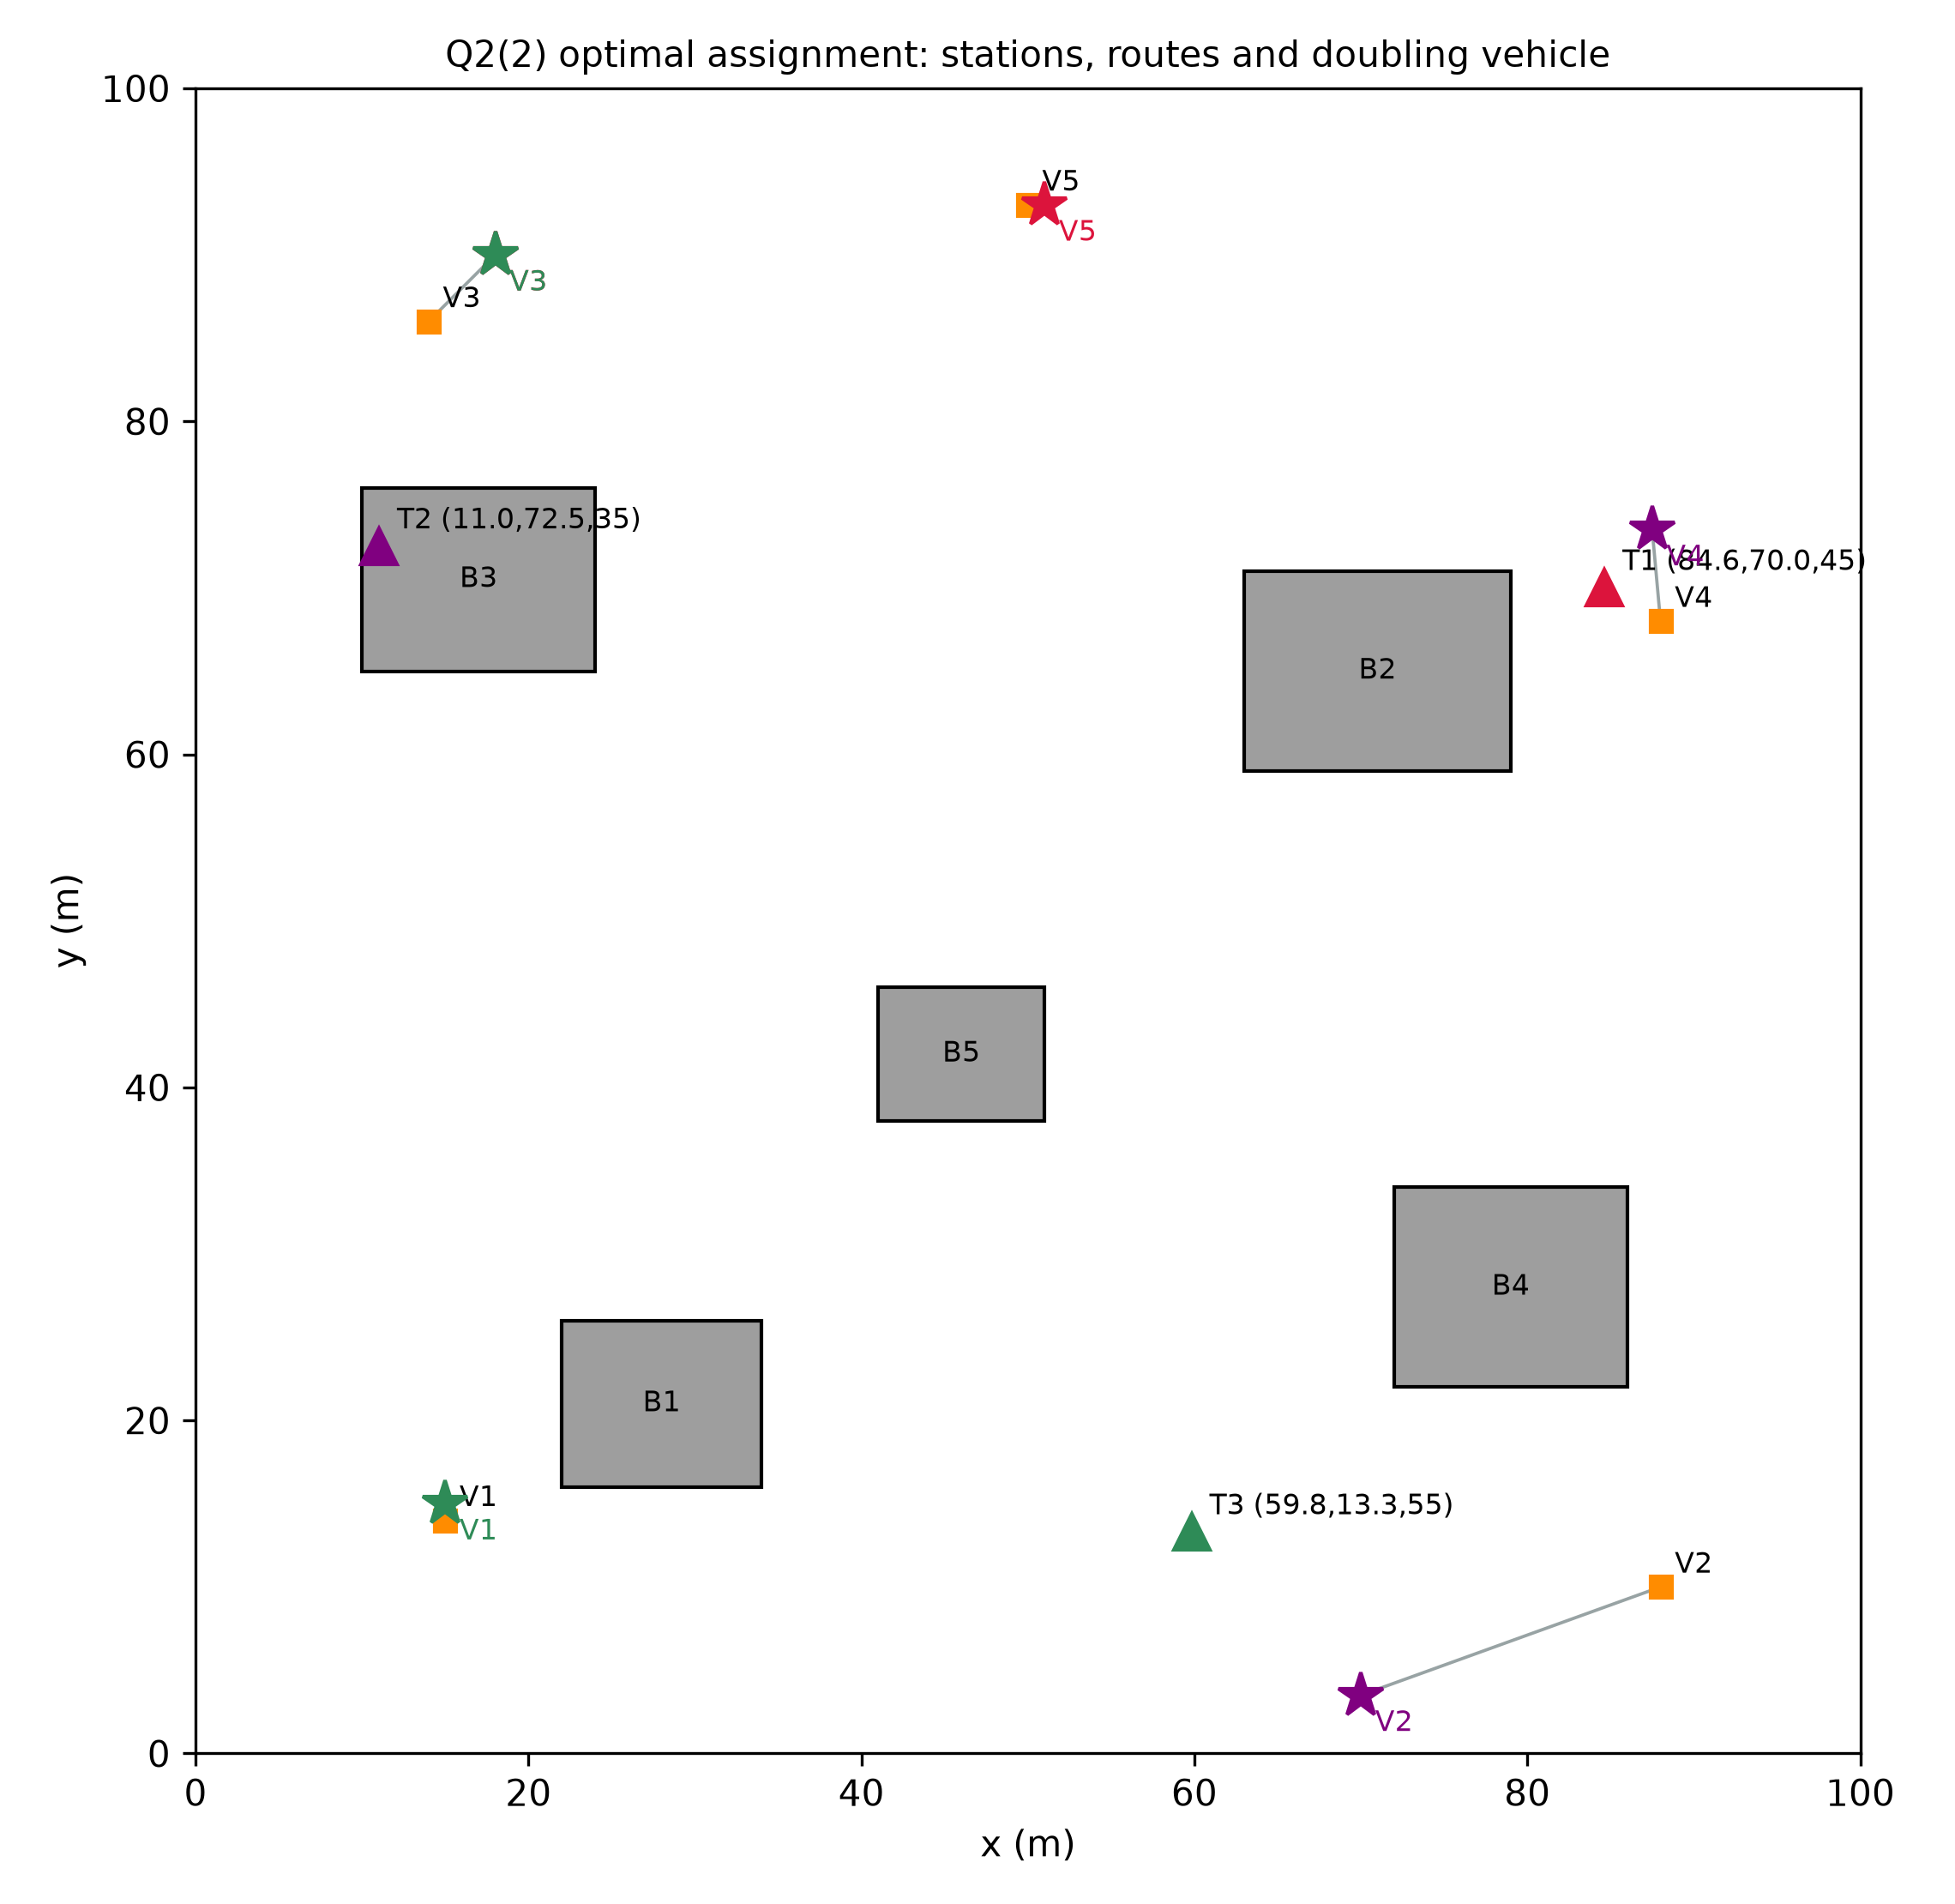
\includegraphics[width=0.42\textwidth]{fig_q2_2_map.png}
\caption{Chosen deployment on the field map: six stations (diamonds) for the three
alerts; V3's two tasks share the single station $(18,90)$, which lies inside both
$\mathcal{F}_{T_1}$ and $\mathcal{F}_{T_3}$, making the second leg zero-travel.}
\label{fig:q2map}
\end{figure}

The optimum found is $t^{*}=11.046\,\mathrm{s}$ with structure ``V3 doubles
$T_1\!\to\!T_3$; V5 partners on $T_1$; V1 partners on $T_3$; V2+V4 serve $T_2$''
(Fig.~\ref{fig:q2map}). Its engine is the shared station $(18,90)$: V3 arrives once,
observes T1 ($2.943$--$7.943\,\mathrm{s}$), resets, and slews in place to T3's bearing
($9.000$--$11.046\,\mathrm{s}$) with \emph{zero} travel---eliminating the round trip that
kills every naive double-task plan. The azimuth-continuous second leg
($343.29^\circ\to298.61^\circ$) also keeps the slew short ($2.046\,\mathrm{s}$).

\begin{table}[!htb]\centering\small
\caption{Per-vehicle event timeline of the chosen schedule (times in s; ``wait'' merges
into obs start where absent).}
\label{tab:q22timeline}
\begin{tabular}{lcccccc}
\toprule
Vehicle--Alert & depart & arrive & ready & obs start & obs end & reset end \\
\midrule
V1--T3 & 0.000 & 0.333 & 1.992 & 11.046 & 16.046 & 17.705 \\
V2--T2 & 0.000 & 6.379 & 10.730 & 10.730 & 15.730 & 20.080 \\
V3--T1 & 0.000 & 1.886 & 2.943 & 2.943 & 7.943 & 9.000 \\
V3--T3 & 9.000 & 9.000 & 11.046 & 11.046 & 16.046 & 18.093 \\
V4--T2 & 0.000 & 1.841 & 7.816 & 10.730 & 15.730 & 21.705 \\
V5--T1 & 0.000 & 0.333 & 1.885 & 2.943 & 7.943 & 9.494 \\
\bottomrule
\end{tabular}
\end{table}

Table~\ref{tab:q22timeline}, Fig.~\ref{fig:q2map} and Fig.~\ref{fig:q2ganttbase}a give
the full timeline: alert
starts are $t^{start}_{T_1}=2.943$, $t^{start}_{T_2}=10.730$,
$t^{start}_{T_3}=11.046\,\mathrm{s}$; the makespan (last reset) is $21.705\,\mathrm{s}$.
The binding alert is T3, whose start is set by V3's arrival from T1's observation plus
the in-place slew---not by V1, ready at T3 since $1.992\,\mathrm{s}$. The azimuth gaps
are $17.65^\circ$ ($T_1$), $50.23^\circ$ ($T_2$), $59.21^\circ$ ($T_3$): the problem
requires only distinct azimuths and accuracy is not the objective here, so the small
$T_1$ gap is admissible; its effect is noted in Section~\ref{sec:sens}.

\begin{figure}[!htb]\centering
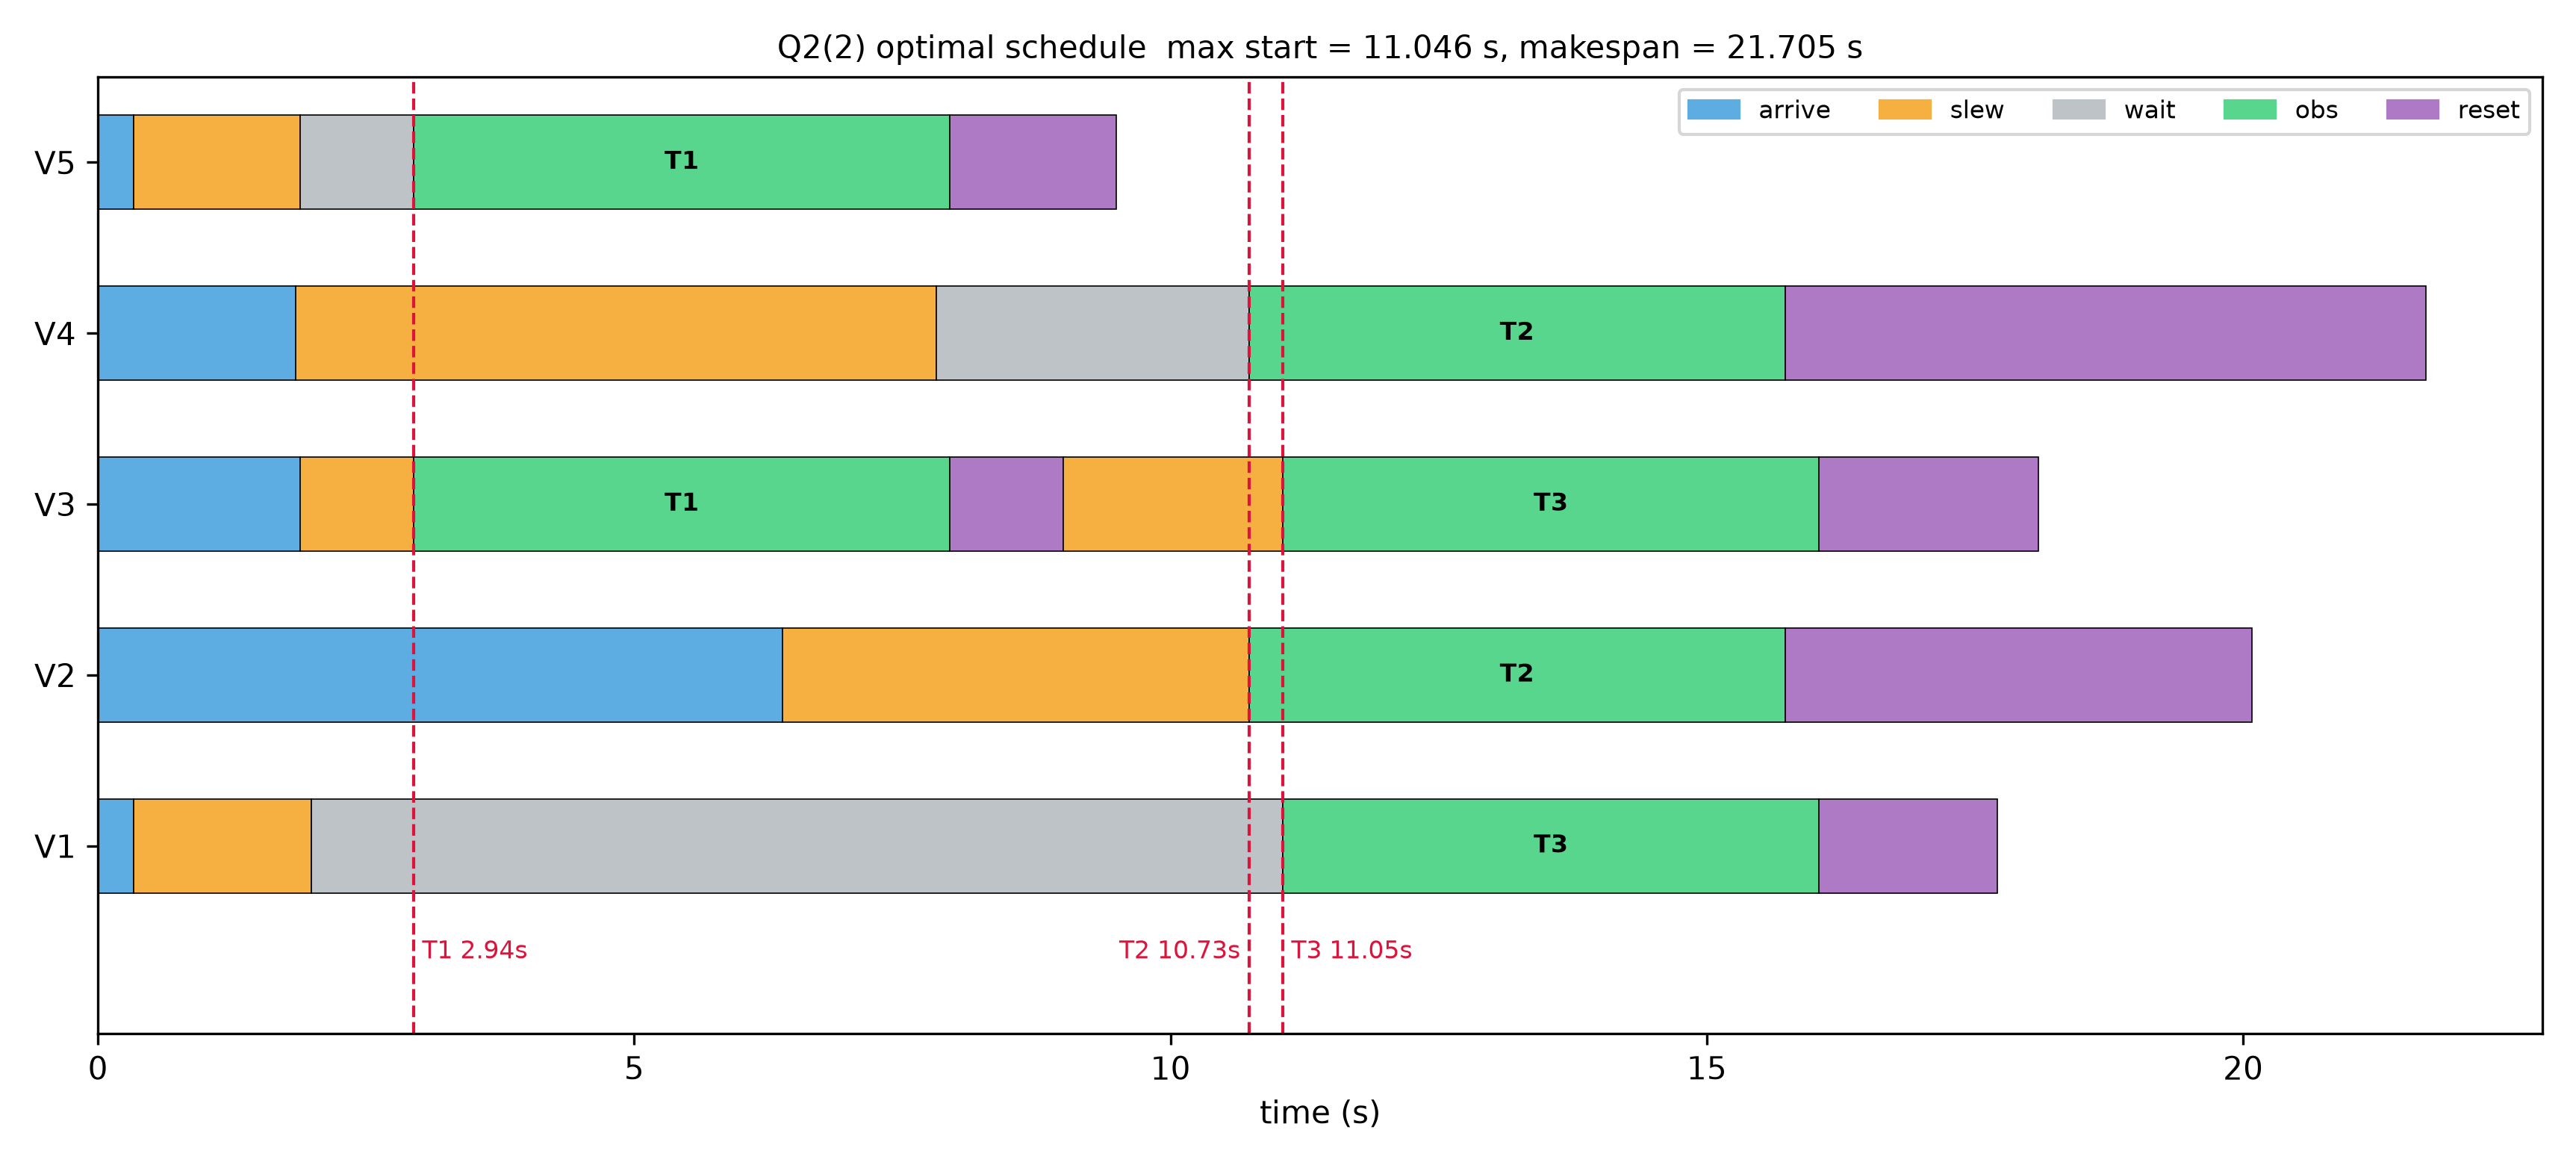
\includegraphics[width=0.49\textwidth]{fig_q2_2_gantt.png}\hfill
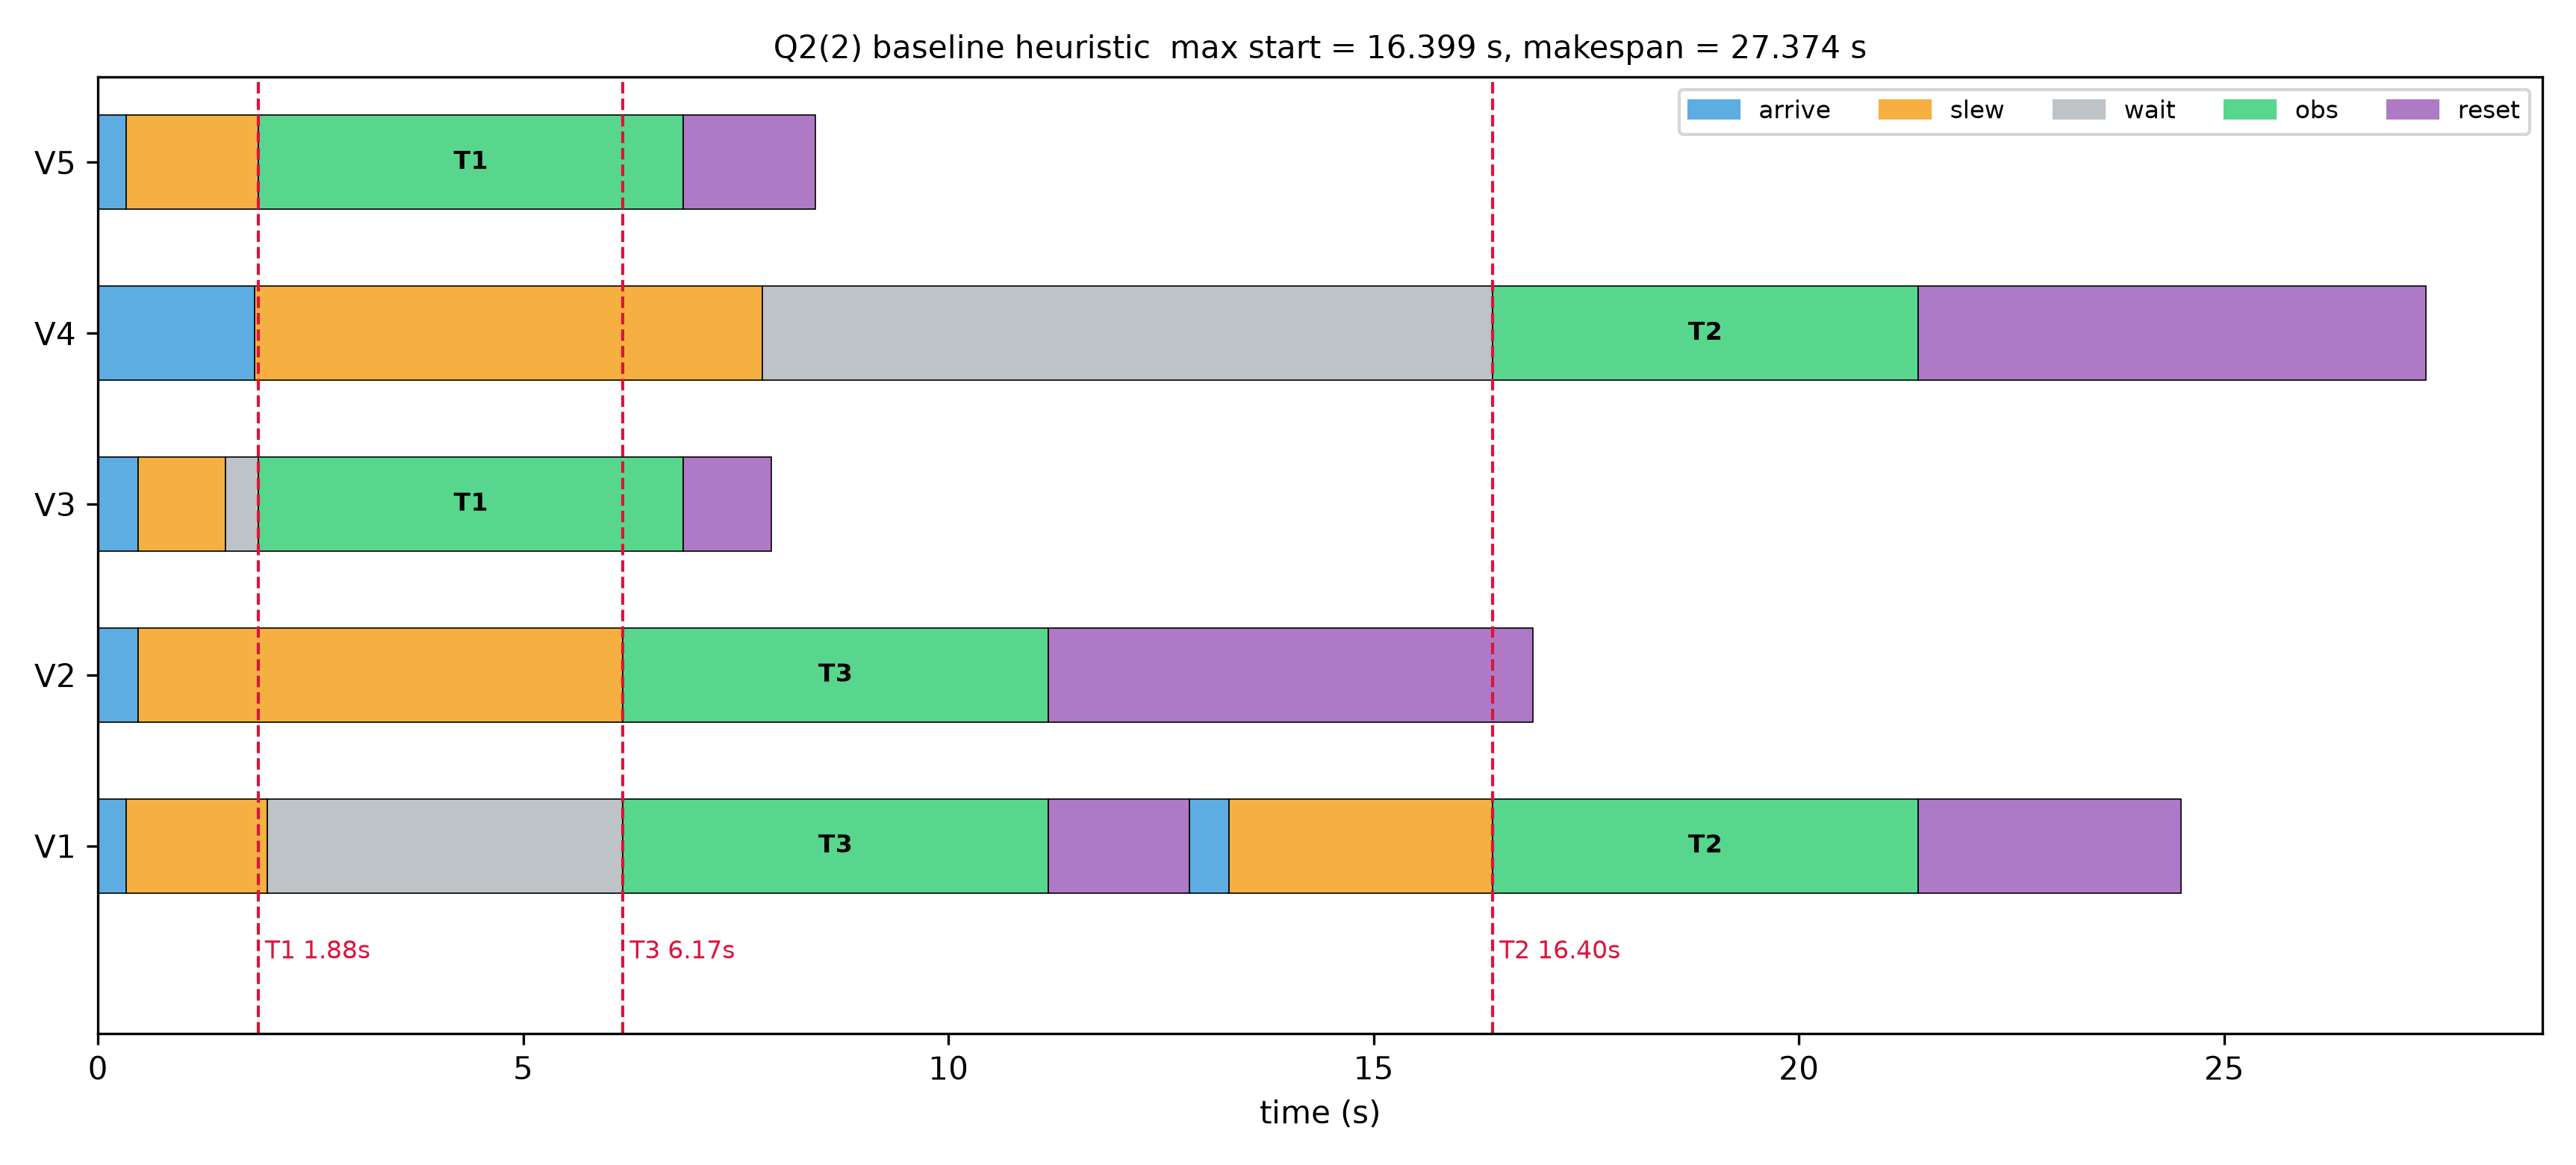
\includegraphics[width=0.49\textwidth]{fig_q2_2_gantt_baseline.png}
\caption{Gantt charts: (a) the chosen schedule; (b) the nearest-assignment baseline,
where V1 doubles $T_3\!\to\!T_2$ and $T_2$---whose independent minimax stations look
attractive locally---starts at $16.399\,\mathrm{s}$, setting the baseline's max.}
\label{fig:q2ganttbase}
\end{figure}

\textbf{Baseline comparison.} The baseline attains $t^{*}=16.399\,\mathrm{s}$: per-alert
starts $T_1$ $1.885$ (equal to its standalone lower bound), $T_3$ $6.172$, $T_2$
$16.399\,\mathrm{s}$. Our schedule improves the max by $5.352\,\mathrm{s}$
($32.6\%$) while individually \emph{losing} on $T_1$ ($-1.058\,\mathrm{s}$) and $T_3$
($-4.875\,\mathrm{s}$)---the signature of the min--max objective, which trades per-alert
excellence for balance. The root cause of the baseline's failure is step (iii): its
doubling vehicle V1 chooses ``$T_3$ first'' by marginal delay, arrives at $T_2$ only
after a full observe--reset--travel cycle, and drags $T_2$ to $16.399\,\mathrm{s}$;
the greedy station choice of step (i), blind to who will double, concentrates the
fastest vehicle (V1) on two nearby alerts and leaves $T_2$ to the slow partner only.
Our structure enumeration sees this interaction explicitly and moves the double task
onto V3 with a shared station instead.

\textbf{Optimality evidence.} No structure among the 360 (with refinement) beats
$11.046\,\mathrm{s}$, and the valid lower bound is $3.873\,\mathrm{s}$ (per-alert earliest
starts ignoring sharing), so the certified gap is $7.17\,\mathrm{s}$; the bound is weak
because it ignores slew and synchronization, and we report it as such rather than
claiming global optimality.

\subsubsection{Validation}

(1) Constraint compliance was re-checked programmatically: every station inside its
observable region, two distinct vehicles per alert, azimuth gaps $\ge1^\circ$, all
routes feasible (V3's legs audited at $5.657$ m and $0$ m with minimum gaps
$\ge10$ m to inflated obstacles). (2) The timeline of Table~\ref{tab:q22timeline} is the
simulator's own output, replayed event-by-event---no manual arithmetic. (3) Parameter
sensitivity ($\pm10\%$) leaves the optimal \emph{structure} unchanged
(Section~\ref{sec:sens}). \emph{Conclusion: the chosen structure is insensitive to
moderate timing-parameter perturbations---no alternative structure overtakes it within
the tested ranges---so the schedule is robust as well as fast.}
